%-----------------------------------------
% Note: Use pdflatex to process this file.
%-----------------------------------------

\documentclass[11pt]{article}
%%\documentclass{book}
\usepackage{geometry}            % See geometry.pdf to learn the layout options. There are lots.
\usepackage{xspace}
\geometry{letterpaper}           % ... or a4paper or a5paper or ... 
%\geometry{landscape}            % Activate for for rotated page geometry
%\usepackage[parfill]{parskip}   % To begin paragraphs with an empty line rather than an indent
\usepackage{graphicx}
\usepackage{amssymb}
\usepackage{alltt}
%\usepackage{epstopdf}
%\DeclareGraphicsRule{.tif}{png}{.png}{`convert #1 `dirname #1`/`basename #1 .tif`.png}
\usepackage[T1]{fontenc}   % so _, <, and > print correctly in text.
\usepackage[strings]{underscore}    % to use "_" in text

\usepackage{hyperref}

%---------------------------------------------------------------------------------

\newcommand{\sref}[1]{$\S$\ref{#1}}
\newcommand\ttcmd{\begingroup\catcode`\_=11 \catcode`\%=11 \dottcmd}
\newcommand\dottcmd[1]{\texttt{#1}\endgroup}
\newcommand{\Begineq}{\begin{equation}}
\newcommand{\Endeq}{\end{equation}}
\newcommand{\fig}[1]{Figure~\ref{#1}}
\newcommand{\vn}{\ttcmd}           
\newcommand{\Th}{$^{th}$\xspace}
\newcommand{\Newline}{\hfil \\}

\newlength{\dPar}
\newlength{\ExBeg}
\newlength{\ExEnd}
\setlength{\dPar}{1.5ex}
\setlength{\ExBeg}{-\dPar}
\addtolength{\ExBeg}{-0.5ex}
\setlength{\ExEnd}{-\dPar}
\addtolength{\ExEnd}{-0.0ex}

\newenvironment{example}
  {\vspace{\ExBeg} \begin{alltt}}
  {\end{alltt} \vspace{\ExEnd}}

%---------------------------------------------------------------------------------

\setlength{\textwidth}{6.25in}
\setlength{\hoffset}{0.0in}
\setlength{\oddsidemargin}{0.25in}
\setlength{\evensidemargin}{0.0in}
\setlength{\textheight}{8.5in}
\setlength{\topmargin}{0in}

\setlength{\parskip}{\dPar}
\setlength{\parindent}{0ex}

%---------------------------------------------------------------------------------

\title{ Synrad Information}
\author{}
\date{October 1, 2010}

\begin{document}
\maketitle

%------------------------------------------------------------------
\section{Introduction} 

Synrad is a program for calculating the synchrotron radiation power
deposition on the beam chamber walls in a storage ring or
accelerator. Synrad works by tracking photons from creation at the
beam to absorption at the chamber wall. The tracking is confined to
the horizontal plane.  Reflections from the wall are not considered.
The vertical extent of the radiation stripe at the wall, important for
calculating the power deposition per unit area, is calculated using
the vertical emittance.

The chamber wall is specified in the horizontal plane by a set of
vertex points with a straight line between points. Exit and entrance
lines like x-ray beam lines or dumps can be modeled in
Synrad. Shadowing of parts of the wall by other parts is taken into
account in the calculation.

Synrad output includes power deposition per longitudinal length, per
unit area on the beam center line, and photon flux. The beam orbit is
not constrained to be zero so calculations to see the affect of
varying the orbit are possible.

Synrad is not to be confused with another program called Synrad3D.
The Synrad3D program uses Monte Carlo to generate photons along with a
full three dimensional chamber model along with a model for the
scattering the photons. The advantage of using Synrad is that it is
quick and accurate since it does not rely on Monte Carlo methods.

Synrad uses the Bmad subroutine library for relativistic
charged-particle simulations\cite{b:bmad} for some of the
calculations. 

%------------------------------------------------------------------

  \begin{figure}[tb]
  \begin{center}
  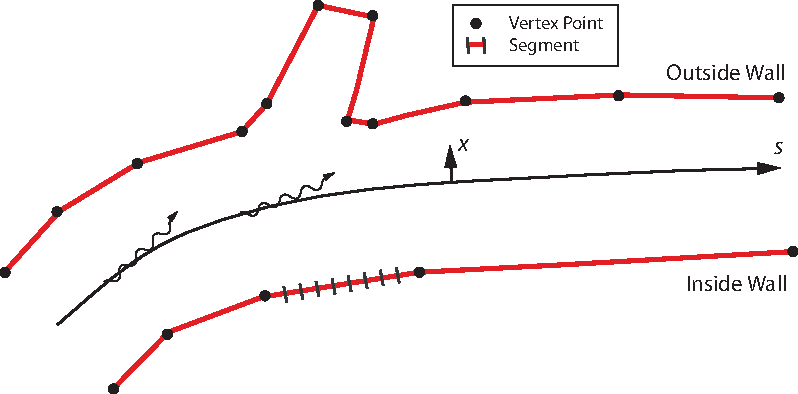
\includegraphics[width=5in]{wall.pdf}
  \caption{
Photon tracking is in the horizontal $x$-$s$ plane. The wall is
divided into an inside part and an outside part. The wall is defined
by a number of vertex points (shown as circles) with straight lines
between vertices. For the calculation, the straight lines are divided
into a number of roughly equal length short segments as shown for
a portion of the inside wall.
  }
  \label{f:wall}
  \end{center}
  \end{figure}

%------------------------------------------------------------------
\section{Simulation Technique} 

Photon generation is based on the standard synchrotron radiation
formulas, applicable for dipoles quadrupoles, and wigglers. The
radiation is assumed to be incoherent, so Synrad cannot treat
undulator radiation. 

Photons are generated roughly uniformly along the length of any
element where photons are produced. The generated photons are tracked
to the vacuum chamber wall. Tracking is confined to be in the
horizontal plane.  The power $P_b$ per unit angle bend of the particle
beam trajectory is\cite{b:sands}
\begin{equation}
  P_b \, \mbox{(W/radian)} = 14.3 \cdot 10^3  \, I_b \, \mbox{(Amps)} \, 
  [E_b \, \mbox{(eV)}]^4 \, [g \mbox{(1/m)}] 
\end{equation}
where $I_b$ is the beam current, $E_b$ is the beam energy, and $g =
1/R$ is the inverse of the bending radius. The power $P_{w1}$ per unit
wall length is then
\begin{equation}
  P_{w1} \, \mbox{(W/m)} = P_b \, \frac{\sin\theta_g}{L_p (m)}
\end{equation}
where $\theta_g$ is the grazing angle between the photon and the wall
and $L_p$ is the length the photon travels from generation to the wall.
The power $P_{w2}$ per unit area on the wall centerline is
\begin{equation}
  P_{w2} \, \mbox{(W/m$^2$)} = \frac{P_{w1}}{2 \, \pi \, \sigma_y}
\end{equation}
where $\sigma_y$ is the effective vertical sigma of the photon distribution at the wall 
\begin{equation}
  \sigma_y^2 = [\epsilon_y \, \beta_y] + [(\epsilon_y \, \gamma_y + 1 / \gamma^2) \, L_p^2]
\end{equation}
where $\beta_y$ and $\gamma_y$ are Twiss parameters, $\epsilon_y$ is
the vertical beam emittance, and $\gamma$ is the usual beam
relativistic factor. The first term in square brackets on the RHS of
the equation is the particle beam height and the second term is due to
the finite vertical opening angle of the photons.

Note: If the lattice is circular, photons leaving one end of the
lattice will be tracked through from the other end. That is, such
photons will be handled correctly. If the lattice is not circular,
photons reaching the ends of the lattice will be absorbed by the wall
there.

Since Synrad is only tracking in the horizontal plane, the vacuum
chamber wall is divided into an ``inside'' section and an ``outside''
section as shown in Fig.~\ref{f:wall}. The ``outside'' section is
defined as the wall on the positive $x$ side of the centerline. The
curvilinear coordinate system used by Synrad corresponds to the Bmad
standard (see the Coordinates chapter in the Bmad
manual\cite{b:bmad}). If there are no vertical bends, the $y$-axis is
in the vertical direction, the $s$-axis is along the direction of the
beam and the $x$-axis is in the horizontal plane.

The inside and outside walls are specified by a number of vertex
points with straight lines between vertex points. Since the coordinate
system is curvilinear, sections of the wall can be curved. For
example, if two vertex points are within a bend, and both vertex
points have the same $x$ value, the ``line'' between them, which has
constant $x$, is actually the arc of a circle. 

For the calculation, the lines between vertex points are broken up
into roughly equal length segments. Note that while Synrad
tries to make segments of equal size, since the distance between
vertex points may not be commensurate with the desired segment length,
the actual segment length can vary from segment to segment.

For a given element where radiation is produced, a set of $N$ photons
are generated and tracked. For wiggler radiation, the number of
photons produced per period of beam oscillation must be of order 10 or
more for an accurate calculation.  Each pair $(i, i+1)$ of photons, with
$i = 1, \ldots, N-1$, defines a section of the beam trajectory over which
radiation is produced.
The $i^{\mbox{th}}$ photon strikes
the wall at wall segment $W_i$. 
For each radiation section, the power incident on the wall segments between $W_i$
and $W_{i+1}$ is computed using interpolation. It is assumed that the
segment length is small enough so that power on a segment is
\begin{equation}
  P_s = l_s \, P_{s0}
\end{equation}
where $P_s$ is the integrated power over the segment, $l_s$ is the
segment length, and $P_{s0}$ is the power density at the center of the
segment. A check is made to see if any segments are shielded from the
photon flux by other parts of the wall. If so, the power on these
segments due to the radiation section is set to zero.

%------------------------------------------------------------------
\section{Main Input File} 

The main input file can be specified on the command line invoking Synrad3d.
If not given, the default name for the main input file is ``\vn{synrad.init}''.
Example main input file:
\begin{example}
  &synrad_params
    sr_param%lat_file = "lat.bmad"   ! Input lattice.
    sr_param%i_beam = 0.1            ! Single-beam current.
    sr_param%epsilon_y = 10e-12      ! Vertical emittance.
    sr_param%n_slice = 20            ! # of slices per element or wiggler period
    seg_len = 0.1                    ! Segment length for calculation.
    beam_direction = 0               ! -1 = track backwards only,
                                     !  0 = track both directions, 1 = forward.
    wall_file = "wall.dat"           ! Name of file specifying the wall.
    forward_beam  = "POSITRON"       ! "POSITRON" or "ELECTRON"
    backward_beam = "ELECTRON"       !  This is important if there are elsep elements.
    use_ele_ix = 0   ! If using only a single element, this is the element index number to use
          ! Otherwise, use 0 for power from all elements
  /
\end{example}
 Fortran namelist input is used.  The tag \vn{"\&synrad_params"}
marks the start of the namelist and the namelist ends with the slash
\vn{"/"} tag. Anything outside of this is ignored. Within the
namelist, anything after an exclamation mark \vn{"!"} is ignored,
including the exclamation mark.

  \begin{description}
  \item[\vn{sr_param\%lat_file}] \Newline
The \vn{lat_file_name} parameter specifies the lattice file to be
used.  Lattices are in Bmad standard format~\cite{b:bmad}. XSIF files may
be used by prefixing the lattice name with the string ``xsif::''.
  \item[\vn{sr_param\%i_beam}] \Newline
The \vn{i_beam} parameter specifies the current (Amps) in a single beam.
  \item[\vn{sr_param\%epsilon_y}] \Newline
The \vn{epsilon_y} parameter specifies the vertical emittance to use 
in the simulation.
  \item[\vn{sr_param\%n_slice}] \Newline
The \vn{n_slice} parameter specifies the number of slices to divide
magnetic elements into.  More slices gives a more accurate depiction 
of the radiation but increases the computation time and file sizes. 
For periodic type wigglers \vn{n_slice} is taken to be the
number of slices per period. For map type wiggler the number of slices is
taken to be equal to the value of the \vn{num_steps} parameter.
  \item[\vn{sr_param\%seg_len}] \Newline
The \vn{seg_len} parameter sets the maximum size of a wall segment. 
A smaller size can give better power deposition resolution but 
increases the computation time. and the output file size.
  \item[\vn{beam_direction}] \Newline
The \vn{beam_direction} parameter specifies the direction of the
tracking to use: -1 = track backwards only (This corresponds to e$^-$
in CESR), 1 = track forward only (e+ in CESR), and 0 = track both
directions.
  \item[\vn{wall_file}] \Newline
The \vn{wall_file} parameter specifies a file giving a list of
x inside, x outside, and s vertices to define the horizontal aperture 
of the wall. See below for more details.
  \item[\vn{forward_beam}] \Newline
The \vn{forward_beam} parameter specifies which species moves in the
positive s direction.  Should be "POSITRON" for CESR. This parameter
only matters if there are \vn{elsep} elements in the lattice.
  \item[\vn{backward_beam}] \Newline
The \vn{backward_beam} parameter specifies which species moves in the
negative s direction.  Should be "ELECTRON" for CESR. This parameter
only matters if there are \vn{elsep} elements in the lattice.
  \item[\vn{use_ele_ix}] \Newline
The \vn{use_ele_ix} parameter specifies the index a single element 
from which to generate synchrotron radiation.  If this is 0, then
generate power from all bends, quads and wigglers.
  \end{description}

%------------------------------------------------------------------
\section{Vacuum Chamber Wall Definition} 

Wall files define a series of wall vertices.  The definition 
includes the s position (meters), and the corresponding 
inside and outside wall offsets at that location (meters).
Note: The s-position of the last vertex will be automatically
set to the $s$ value at the end of the lattice.

Example:
\begin{verbatim}
! Note: x_inside should be negative.
! Note: First s_position should be 0.
!
!s_position   x_inside   x_outside
        0       -0.025  0.025
        10      -0.025  0.025
        10.3    -0.025  0.037
        ... etc ...
\end{verbatim}

%------------------------------------------------------------------
\section{Output Files} 

There are five output files generated:
\begin{verbatim}
  element_power.dat
  synch_power_negative_x_side.dat
  synch_power_positive_x_side.dat
  synrad_negative_x_side.txt
  synrad_positive_x_side.txt
\end{verbatim}

  \begin{description}
  \item[\vn{element_power.dat}] \Newline
List of all elements where radiation is produced showing the power radiated and
the power that hit the walls. These two numbers should be the same.
  \item[\vn{synch_power_negative_x_side.dat}, \vn{synch_power_positive_x_side.dat}] \Newline
List of all wall segments showing such things as power deposited, power per unit length, photons
per second impinging, etc.
  \item[\vn{synrad_negative_x_side.txt}, \vn{synrad_positive_x_side.txt}] \Newline
Similar to the \vn{synch_power*.dat} files.
  \end{description}


%------------------------------------------------------------------
\begin{thebibliography}{9}

\bibitem[Bmad]{b:bmad}
D. Sagan,
"Bmad: A Relativistic Charged Particle Simulation Library"
Nuc.\ Instrum.\ \& Methods Phys.\ Res.\ A, {\bf 558}, pp 356-59 (2006).

The Bmad Manual can be obtained at:\hfill\break
\hspace*{20pt} http://www.lepp.cornell.edu/$\scriptstyle\sim$dcs/bmad

  \bibitem[Sands]{b:sands}                                      
Matthew Sands, {\em The Physics of Electron Storage Rings, An Introduction},
SLAC-121 Addendum, 1970.

\end{thebibliography}

\end{document}  
